There are various of different gradient descent algorithms. As mentioned in the backpropagation section, gradient descent is a technique which measures the degree of change w.r.t some parameter, at a certain point in a function. It is an iterative process that makes it path towards some minimum. This minimum point is defined as the local minima of the function; it is not necessarily a global minima. This means, gradient descent can be applied on functions which are differentiable w.r.t its parameters. This, makes gradient descent a relatively effiecient optimization method, when looking at neural networks.\\

\noindent
There are variations of how the gradient descent is done, one of which is the Stochastic gradient descent (SGD) algorithm. When training on some dataset, usually what the programmer does is using batches, which refers to the number of samples in the dataset, which is used to calculate the gradient. Using the gradient of all individual samples results in a smoother way of finding the minima. Though, if the dataset is very big, this can quickly become a very comprehensive task. SGD relies on the random probability of randomly picking one sample from the batch in each iteration. This means that SGD takes a single example of a gradient, instead of the sum of all gradients of the error function. As can be seen in figure(~\ref{fig:image2}), Doing this results in a more noisy way of finding the local minima. The noisy path doesn't matter, as long as the path it takes in finding the local minima, is actually finding the correct local minima. It's important to note, that because of the stochastic probability of picking some gradient, it is required that a lot of data is available.

\begin{figure}[h]
\centering
\begin{subfigure}{0.4\textwidth}
\centering
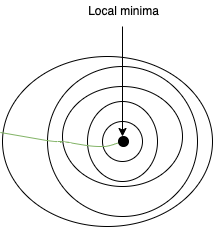
\includegraphics[scale=0.4]{latex/imgs/GDsmooth.png}
\caption{GD on each individual sample\\  in the dataset}
%\label{fig:subim1}
\end{subfigure}
\begin{subfigure}{0.4\textwidth}
\centering
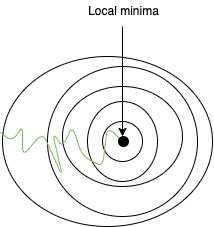
\includegraphics[scale=0.4]{latex/imgs/SGDpath.png}
\caption{SGD's path using randomly \\ selected gradient}
%\label{fig:subim2}
\end{subfigure}
\caption{Two different gradient descent paths}
\label{fig:image2}
\end{figure}
